\scanpage{121}
\mspage{120}


6) Suppose now that $C$ is an \deleted{additive}\inserted{abelian} $k$-linear category ($k$ a field) equipped with a faithful exact functor $F:C\handwritten{\to}\mathrm{Modf}(k)$, so that $C$ identifies with the category of finite \inserted{(continuous)\handwritten{\begin{tikzpicture}[x=.55cm,y=.55cm,baseline=-.2ex]\draw (0,-.23) .. controls (.04,-.04) and (.14,.05) .. (.38,.05)--(1.8,.06) .. controls (2,.07) and (2.12,.2) .. (2.12,.42);\end{tikzpicture}}} representations \deleted{of a} of a profinite algebra $U$ over $k$\inserted{(associative, unital)\handwritten{\begin{tikzpicture}[x=.55cm,y=.55cm,baseline=-.2ex]\draw (0,-.23) .. controls (.04,-.04) and (.14,.05) .. (.38,.05)--(1.8,.06) .. controls (2,.07) and (2.12,.2) .. (2.12,.42);\end{tikzpicture}}}, or of comodules over the \inserted{topological\handwritten{\begin{tikzpicture}[x=.55cm,y=.55cm,baseline=-.2ex]\draw (0,-.23) .. controls (.04,-.04) and (.14,.05) .. (.38,.05)--(1.8,.06) .. controls (2,.07) and (2.12,.2) .. (2.12,.42);\end{tikzpicture}}} dual $A$ of $k$, which is a coalgebra (associative, unital). Then the datum of a \inserted{bilinear\handwritten{\begin{tikzpicture}[x=.55cm,y=.55cm,baseline=-.2ex]\draw (0,-.23) .. controls (.04,-.04) and (.14,.05) .. (.38,.05)--(1.8,.06) .. controls (2,.07) and (2.12,.2) .. (2.12,.42);\end{tikzpicture}}} functor $\unsure{\otimes|\Omega}$ compatible with $F$ (i.e. for which \deleted{it is} one has \uline{equality} $F(X\otimes Y)=F(X)\otimes F(Y)$\handwritten{)} \uline{is equivalent} to the datum of a diagonal morphism $U\handwritten{\to}U\overset{\handwritten{\scriptscriptstyle\wedge}}{\otimes}_k U$, or again of a multiplication law on $A$. \unsure{\rlap{\begin{tikzpicture}[x=1em,y=1em,baseline=0pt]\draw[line width=1pt] (.7,.73)--(1.03,.73);\draw[line width=1pt] (.85,.72)--(.85,.95);\fill (1.15,.72)--(1.29,.72)--(1.28,.99)--(1.22,.91)--(1.14,.94)--cycle;\end{tikzpicture}}An|An} additional datum (in the sense of 4)) a) \deleted{b)}\inserted{\handwritten{b)}} or c) \uline{compatible} with $F$, $c=\mathrm{id}$ is then uniquely determined, if it exists.\handwritten{\llap{\raisebox{-.65ex}{,}}}\inserted{\handwritten{\deleted{\unsure{for b)} \unsure{it} \illegible{4} \unsure{that there be an} $\unsure{\epsilon|e}:U\to k$ (\unsure{homomorphism of $k$-algebras}) i.e. $\epsilon\in A$ \unsure{and that it be}}}\handwritten{
\begin{tikzpicture}[x=.55cm,y=.55cm,baseline=-.2ex]\draw (-.15,-.3) .. controls (.02,.06) and (.16,.1) .. (.45,.08)--(2.45,.02);\draw (2.5,.03) .. controls (2.58,-.18) and (2.62,-.24) .. (2.78,-.24);\end{tikzpicture}}} It exists if and only if $A$ is associative, resp. unital resp. commutative. When these conditions are satisfied simultaneously, we thus have an affine \deleted{group}\inserted{\handwritten{monoid}} scheme over $k$, which allows the situation to be reconstructed. - If we likewise have $\mathbb{C}',F'$ over the same $k$, \deleted{with a $\otimes$,} then the functors $G:C\handwritten{\to} C'$ compatible with $F,F'$ correspond exactly to the homomorphisms of topological $k$-algebras $U'\handwritten{\to}U$, or of $k$-coalgebras $A\handwritten{\to}A'$. If $\mathbb{C}$ and $C'$ are equipped with bilinear structures $\otimes\unsure{\rlap{\handwritten{
\begin{tikzpicture}[x=1em,y=1em,baseline=0pt]\draw[line width=.6pt] (.48,.9) .. controls (.24,.55) and (.28,.15) .. (.22,-.18);\draw[line width=.6pt] (.22,-.18) .. controls (.37,.15) and (.64,.35) .. (.82,.53);\end{tikzpicture}}}x|\deleted{x}\handwritten{/}}\otimes$, then the functor $G$ is a $\otimes$-functor with an isomorphism $c$ tra\rlap{e}nsformed by $F'$ into $\mathrm{id}$ (which suffices to characterize \deleted{it}\inserted{\handwritten{$c$\begin{tikzpicture}[x=.45cm,y=.45cm,baseline=-.2ex]\draw (0,-.35) .. controls (.02,-.04) and (.08,.1) .. (.3,.14)--(.7,.16) .. controls (.88,.18) and (.94,.32) .. (.95,.58);\end{tikzpicture}}} then) if and only if $U'\handwritten{\to}U$ is compatible with the diagonals i.e. $A\handwritten{\to}A'$ is compatible with the mu\rlap{\handwritten{l}}t\rlap{\handwritten{t}}liplications. Any additional structures a)\deleted{, b)} or c) are respected automatically,\inserted{\handwritten{for b) one must \unsure{impose|assume} compatibility with the augmentations of $U$ resp. with the units of $A,A'$}}

\margin{generalize at least partially to the case of a $k$ which is not a field}

\margin{\figure{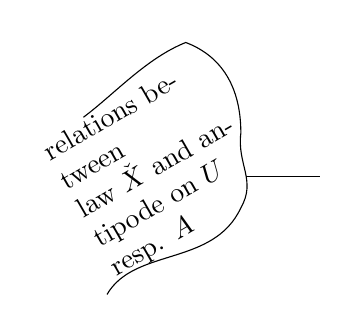
\begin{tikzpicture}[baseline]
\draw (0,0) .. controls (.35,.6) and (1.35,.35) .. (1.7,1.1) .. controls (1.9,1.45) and (1.65,1.65) .. (1.7,2.05) .. controls (1.7,2.7) and (1.4,3.05) .. (1,3.2) .. controls (.5,3) and (.1,2.55) .. (-.3,2.25);
\draw (1.76,1.5)--(2.7,1.5);
\node[rotate=30,align=left,text width=2.65cm] at (.8,1.7) {\handwritten{relations between\\law $\check{X}$ and antipode on $U$\\resp. $A$}};
\end{tikzpicture}}}

\figure{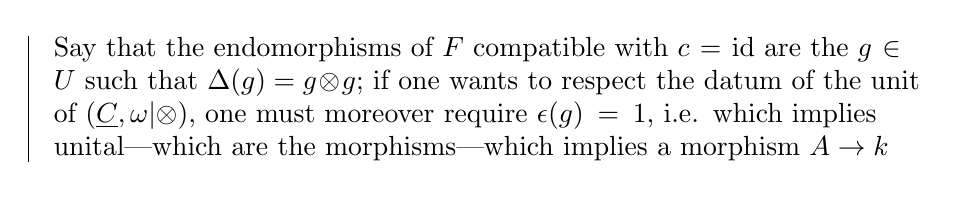
\begin{tikzpicture}[baseline]
\draw (0,0)--(0,1.6);
\node[anchor=west,align=left,text width=11cm] at (.2,.8) {\handwritten{Say that the endomorphisms of $F$ compatible with $c=\mathrm{id}$ are the $g\in U$ such that $\Delta(g)=g\otimes g$; if one wants to respect the datum of the unit of $(\underline{C},\unsure{\omega|\otimes})$, one must moreover require $\epsilon(g)=1$, i.e. \unsure{which implies unital|which are the morphisms|which implies a morphism} $A\to k$}};
\end{tikzpicture}}

7) A\unsure{\rlap{\begin{tikzpicture}[x=1em,y=1em,baseline=0pt]\draw[line width=.4pt] (.05,-.05) .. controls (-.07,-.13) and (.07,-.25) .. (.2,-.08)--(.35,.04);\draw[line width=.4pt] (.2,-.08)--(.16,-.28);\draw[line width=.4pt] (.36,.01)--(.42,-.2);\end{tikzpicture}}n|n} example. We take for $C$ the category of graded\deleted{\unsure{s}} modules over a commutative ring $\mathbb{k}$, with the ordinary graded tensor product and as unit the module $\mathbb{k}_s$ graded in degree zero, datum\deleted{s di} of $u$ and $v$ as usual, as well as $\handwritten{\phi}$ (associativity) and $\handwritten{\unsure{\mu|\psi}}$ (commutativity). All the axioms of number 1 are satisfied, and the forgetful functor (with $c=\mathrm{id}$) isna $\otimes$-functor respecting all the data a)b)c). Thus if $k$ is
